The project also provides an educational and research platform beyond the competition. In particular, in-flight assessment of a phased array extends University of Hartford microwave/metamaterial research toward a realistic mobile communication environment. A successful outcome is not just reaching the altitude target; it includes collecting interpretable RF and flight data and safely recovering the hardware for inspection and reuse.

Beyond its competition objectives, A.R.E.S. serves as an educational and research platform developed in collaboration with the University of Hartford's Multiscale Metamaterial Research Laboratory. This collaboration integrates the laboratory's ongoing research in microwave and metamaterial technologies into the P.H.O.B.O.S. phased-array antenna payload, extending laboratory-based research into a dynamic, real-world flight environment. By evaluating the performance of an electronically steered antenna aboard a sounding rocket, the project aims to advance research into directional communication systems for future aerospace applications. Consequently, mission success is defined not only by achieving the competition altitude target, but also by collecting meaningful RF and flight-performance data and safely recovering the vehicle and experimental hardware for postflight analysis and continued research.
Our practicle scernio should maybe include the CT space grant who is funding the PHOBOS devopment and EBAD who is funding the rocket itself The primary users are AURORA student engineers and faculty researchers who need a repeatable platform for evaluating flight avionics and experimental RF hardware. Secondary stakeholders include competition safety inspectors, range personnel, and future students who will reuse or improve the modular systems. The operating setting is an authorized outdoor high-power rocket range, including launch-pad preparation, ascent to approximately 10,000~ft AGL, descent, recovery, and postflight data analysis."

I would include both funding organizations in the Practical Scenario because they help establish the project's real-world context, stakeholders, and research objectives. I would also connect the PHOBOS payload to the Multiscale Metamaterial Research Laboratory.
Revised Practical Scenario

The primary users of A.R.E.S. are student engineers within the University of Hartford's AURORA Rocketry Club and faculty researchers seeking a reusable platform for evaluating experimental avionics, communication systems, and aerospace technologies. The project is supported by Ensign-Bickford Aerospace & Defense (EBAD), which provides funding for the development and construction of the launch vehicle, and the NASA Connecticut Space Grant Consortium, which funds the development of the P.H.O.B.O.S. phased-array antenna payload. Through collaboration with the University's Multiscale Metamaterial Research Laboratory, the project also provides an opportunity to evaluate microwave and antenna technologies outside the controlled laboratory environment. Additional stakeholders include competition officials, launch-range personnel, and future AURORA members who may continue developing and utilizing the platform.

A representative use case involves preparing A.R.E.S. for launch at the 2027 International Rocket Engineering Competition (IREC) in Midland, Texas. Prior to launch, the team will integrate and verify the vehicle's structural, propulsion, recovery, telemetry, and experimental payload systems. During flight, the rocket will ascend toward its target altitude of approximately 10,000 feet above ground level while the D.E.I.M.O.S. system records and transmits flight telemetry and the P.H.O.B.O.S. payload evaluates electronically steered RF communication with a ground station. The C.O.M.E.T. flight computer will monitor flight conditions and initiate the appropriate parachute deployment events to enable safe recovery. Following the flight, the team will retrieve the vehicle, download recorded data, and compare experimental results against predicted performance. These results will support continued development of the A.R.E.S. platform and the laboratory's research into communication technologies for future aerospace applications.

This version addresses the assignment's who, where, when, and how requirements while explaining how the sponsors and research laboratory contribute to the project. It also presents the launch as a realistic engineering and research mission rather than simply a competition attempt.
Does that really meet the Practical scenrio part ?\subsection{Practical Scenario}
The primary users are AURORA student engineers and faculty researchers who need a repeatable platform for evaluating flight avionics and experimental RF hardware. Secondary stakeholders include competition safety inspectors, range personnel, and future students who will reuse or improve the modular systems. The operating setting is an authorized outdoor high-power rocket range, including launch-pad preparation, ascent to approximately 10,000~ft AGL, descent, recovery, and postflight data analysis.

Prior to launch, the team integrates the three independent electronic subsystems, verifies batteries and connectors, inspects motor and structural hardware, checks continuity of both recovery channels, and verifies GPS acquisition and radio reception from a ground station. The RF team checks antenna matching and beam-control commands before flight; the mechanical team inspects the motor retention, parachutes, shock cords, and mounting interfaces. Recovery electronics remain inhibited until the appropriate launch preparation stage and are armed under the applicable range procedure \cite{tripoliCode}.

Following an approved launch, \deimos{} records position and attitude and transmits available telemetry to the ground station. In parallel, \phobos{} sends an experimental 2.4-GHz signal and updates its phase settings to investigate beam direction as the rocket rotates. \comet{} autonomously identifies flight events from its onboard sensors, commands the drogue at apogee, and subsequently commands the main parachute at a proposed altitude of approximately 700~ft AGL. A separate commercial recovery altimeter is planned to meet competition requirements and provide an independent deployment path; the independence and electrical separation must be demonstrated before flight. After landing, the team recovers the vehicle, downloads nonvolatile logs, correlates the RF link measurements with orientation, and compares measured flight behavior with simulation."
…

Yes, your current Practical Scenario meets most of the assignment requirements, but I think it could be improved. Right now, it reads more like a technical flight operations procedure than a practical use case explaining why someone would use A.R.E.S. and what they gain from it.

The assignment specifically asks for:

Requirement
	

Current version
	

Assessment

Purpose — Why is the product being designed?
	

Implied through testing and data collection
	

Needs a more explicit explanation

User/Customer — Who benefits?
	

Identifies AURORA, faculty, and future students
	

Meets requirement

Where — Operating environment
	

Authorized high-power rocket range
	

Meets requirement

When — When is it used?
	

Describes preflight through recovery
	

Could explicitly mention IREC 2027

How — How is it operated?
	

Thorough subsystem operation sequence
	

Meets requirement

Realistic example
	

Describes an actual flight mission
	

Meets requirement

I would preserve most of your technical description, but add the research motivation, funding relationships, and specific competition scenario. Those details establish the practical reason the project exists.
My suggested revision

This is what I would use in your report. It maintains the technical detail while better addressing the assignment.
\subsection{Practical Scenario}

The primary users of \ares{} are student engineers within the
University of Hartford's AURORA Rocketry Club and faculty
researchers seeking a reusable platform for testing experimental
avionics, communication systems, and aerospace technologies.
The project is developed in collaboration with the University's
Multiscale Metamaterial Research Laboratory, with the goal of
extending laboratory research in microwave and antenna
technologies into a realistic flight environment.

Development of the project is supported by Ensign-Bickford
Aerospace \& Defense (EBAD), which provides funding for the
rocket's development, and the NASA Connecticut Space Grant
Consortium, which funds development of the \phobos{} phased-array
antenna payload. Together, these efforts provide an opportunity
to demonstrate experimental communication technologies while
developing the infrastructure and experience necessary for
future student aerospace research.

A representative application of \ares{} is its participation
in the 2027 International Rocket Engineering Competition
(IREC) in Midland, Texas. The competition provides a
structured environment in which the team must design,
construct, test, and launch a sounding rocket targeting
an altitude of approximately 10,000~ft AGL while carrying
an experimental payload. This mission allows the team
to evaluate whether the developed systems can operate
reliably under the acceleration, vibration, rotation,
and environmental conditions experienced during flight.

Prior to launch, the team integrates the vehicle's electronic
subsystems, verifies electrical connections and battery
operation, and inspects the structural and recovery hardware.
The RF team evaluates antenna performance and communication
with the ground station, while the mechanical team verifies
the vehicle's structural interfaces, motor retention,
and recovery equipment. The recovery systems are checked
and armed according to the applicable range safety
procedures \cite{tripoliCode}.

During flight, \deimos{} measures and records the rocket's
position, acceleration, and orientation while transmitting
telemetry to the ground station. Simultaneously, \phobos{}
investigates electronically steered communication using a
2.4-GHz phased-array antenna. By adjusting the relative
phase of its antenna elements in response to the rocket's
orientation, the payload will attempt to maintain a
directional communication link with the receiving ground
station. The resulting measurements will allow researchers
to evaluate phased-array performance under dynamic flight
conditions rather than exclusively within a laboratory.

The \comet{} flight computer monitors onboard sensors
to identify flight events and initiate the dual-parachute
recovery sequence. The drogue parachute is commanded at
apogee, followed by the main parachute at a proposed
altitude of approximately 700~ft AGL. A separate commercial
deployment altimeter is also planned to provide an
independent recovery system.

Following landing, the team recovers the rocket and
downloads the recorded flight data. Measurements from
\deimos{} and \phobos{} are compared to investigate the
relationship between vehicle orientation, antenna steering,
and received signal performance. Flight data is also
compared against simulations to evaluate vehicle performance
and identify potential design improvements.

Success is therefore measured not only by achieving the
competition altitude target and safely recovering the
vehicle, but also by obtaining meaningful experimental
data that supports continued research within the
Multiscale Metamaterial Research Laboratory and future
development of the AURORA program.
Why this is stronger

The important improvement is that the scenario now establishes three connected objectives: competing in IREC, developing a repeatable student research platform, and advancing the laboratory's phased-array communication research.

It also explains why the funding matters. The NASA Connecticut Space Grant supports the scientific experiment, while EBAD supports the rocket platform needed to conduct that experiment.

One thing I would retain from your original is the technical sequence of preflight checks, launch, telemetry, deployment, and recovery. That is exactly the level of detail that makes the scenario credible for a senior engineering capstone.

I would use this revised version for the assignment. It directly answers all five practical-scenario questions without turning the section into a general project introduction.
Pasted text(20261102-040020).txtDocument
Okay we simplfied this down the last version was way too verbose and included liams stuff when we dont need it "
Worked for 38s

Understood. I'll treat this simplified LaTeX file as the new working version of the A.R.E.S. report, rather than the longer version I generated previously.

The focus will remain on Nicholas's embedded systems, sensing, and telemetry investigations and Kyle's phased-array and RF technology investigations. We'll retain the overall A.R.E.S. requirements because they establish the vehicle's design constraints, but avoid an unnecessary standalone mechanical technology investigation.

I noticed a few things in the updated file:

    Leftover Liam content: There's still a paragraph beginning \noindent\textbf{Selected approach:} G12 fiberglass airframe sections... immediately after Kyle's investigation. This can be removed.

    Repeated information: The Overview and Practical Scenario repeat some of the research objectives. We can shorten those sections without sacrificing the assignment requirements.

    Team technology selection: The individual investigations identify selected components, but a brief paragraph summarizing the team's combined decisions would more directly satisfy Step 2.

    Motor mount: The requirements table now specifies 98 mm instead of the previous 75 mm. We should confirm whether that change was intentional.

One assignment consideration: the instructions call for an investigation from each team member. If Liam remains a listed member, omitting his investigation entirely could cost points, even if his mechanical work doesn't need to be expanded in this version.

Going forward, I'll preserve your existing writing, technical choices, and Kyle's table formatting, and make targeted edits rather than expanding the report with unnecessary material.
Assignment 7 System Block Diagram First Draft and Key Principles & Technologies Investigation(1).pdfPDF
This is what another group submitte can you edit the text I sen to follow closer to this excep for that they forgot to inlcude the FBDS
Worked for 4m 56s

I revised your A.R.E.S. report to follow the other group's submission more closely, while retaining your IEEEtran formatting and all three functional block diagram sections.

The report is now 7 pages, including the cover and references, compared with the longer version from earlier.

Download Overleaf Project (ZIP)

LaTeX source and folders for your diagrams

Download Revised LaTeX (.tex)

Preview Compiled Report (PDF)
What I changed

    Use Case: Shortened the overview and practical scenario while retaining the Multiscale Metamaterial Research Laboratory collaboration, NASA Connecticut Space Grant, and EBAD.

    Requirements: Replaced the lengthy specifications tables with concise subsystem requirements, similar to the example.

    FBDs: Preserved three separate figure sections for PHOBOS, DEIMOS, and COMET, using your original image paths.

    Technology investigations: Reorganized Nicholas's and Kyle's research into short explanations followed by feature-by-feature comparison tables.

    Formatting: Retained booktabs, \multirow, and the existing LaTeX packages, with selected technologies clearly highlighted.

    Sources: Kept a reference list with titles and URLs.

I also removed Liam's separate mechanical technology investigation, as requested, while keeping his name and major on the cover.

One assignment concern: The instructions technically require each team member to contribute an investigation. If Liam is submitting as part of this team, you should confirm whether his separate work needs to be included before the final submission.

The PDF compiles successfully. The only missing items are the three individual FBD images, which you can add directly in Overleaf.
ARES_Assignment7_Revised.texFile
ARES_Assignment7_Revised.pdfPDF


\documentclass[11pt]{IEEEtran}

% ========================= Packages (retained) =========================
\usepackage{graphicx}
\usepackage{float}
\usepackage{pgfplots}
\usepackage{pgfplotstable}
\usepackage{csvsimple}
\usepackage{tikz}
\usepackage{circuitikz}
\usepackage{siunitx}
\usepackage{booktabs}
\usepackage{hyperref}
\usepackage{multirow}
\usepackage{tabularx}
\usepackage{nicematrix}
\usepackage{array}
\pgfplotsset{compat=newest}

% ========================= Project Commands =========================
\newcommand{\comet}{C.O.M.E.T.}
\newcommand{\ares}{A.R.E.S.}
\newcommand{\phobos}{P.H.O.B.O.S.}
\newcommand{\deimos}{D.E.I.M.O.S.}
\newcommand{\insight}{INSIGHT}
\newcommand{\RHeight}{12}

\hypersetup{colorlinks=true,linkcolor=black,urlcolor=blue,citecolor=black}
\urlstyle{same}
\setlength{\emergencystretch}{2em}
% FBDs preserve the original user's file paths. When no image has been added,
% the resulting PDF shows an intentional placeholder instead of failing to build.
\newcommand{\showfbd}[2]{%
  \IfFileExists{#1}{%
    \includegraphics[width=0.94\linewidth,height=2.15in,keepaspectratio]{#1}%
  }{%
    \fbox{\parbox[c][1.65in][c]{0.91\linewidth}{\centering
      \textbf{Functional Block Diagram Placeholder}\\[5pt]
      #2\\[7pt]
      \texttt{\detokenize{#1}}\\[5pt]
      Export the individual block diagram to this location.}}%
  }%
}

\begin{document}
\onecolumn

% If you have the existing ARES cover page, it will be used automatically.
\IfFileExists{Documentation/ARES/Title.tex}{%
  %%%%%%%% Needs Project Title, Names of Team Members, Instructors, and Advisors %%%%%%%%%%%%%%%%%

\onecolumn

\newcommand{\Space}{\\[.5cm]}
%\lhead{A.U.R.O.R.A.}
%\chead {}
%\rhead{\comet}
\begin{center}
    \vfill
    \textbf{\Large AURORA Rocket and Experimental Systems (A.R.E.S.)}
\vfill
  \begin{figure}[h]
    \centering
    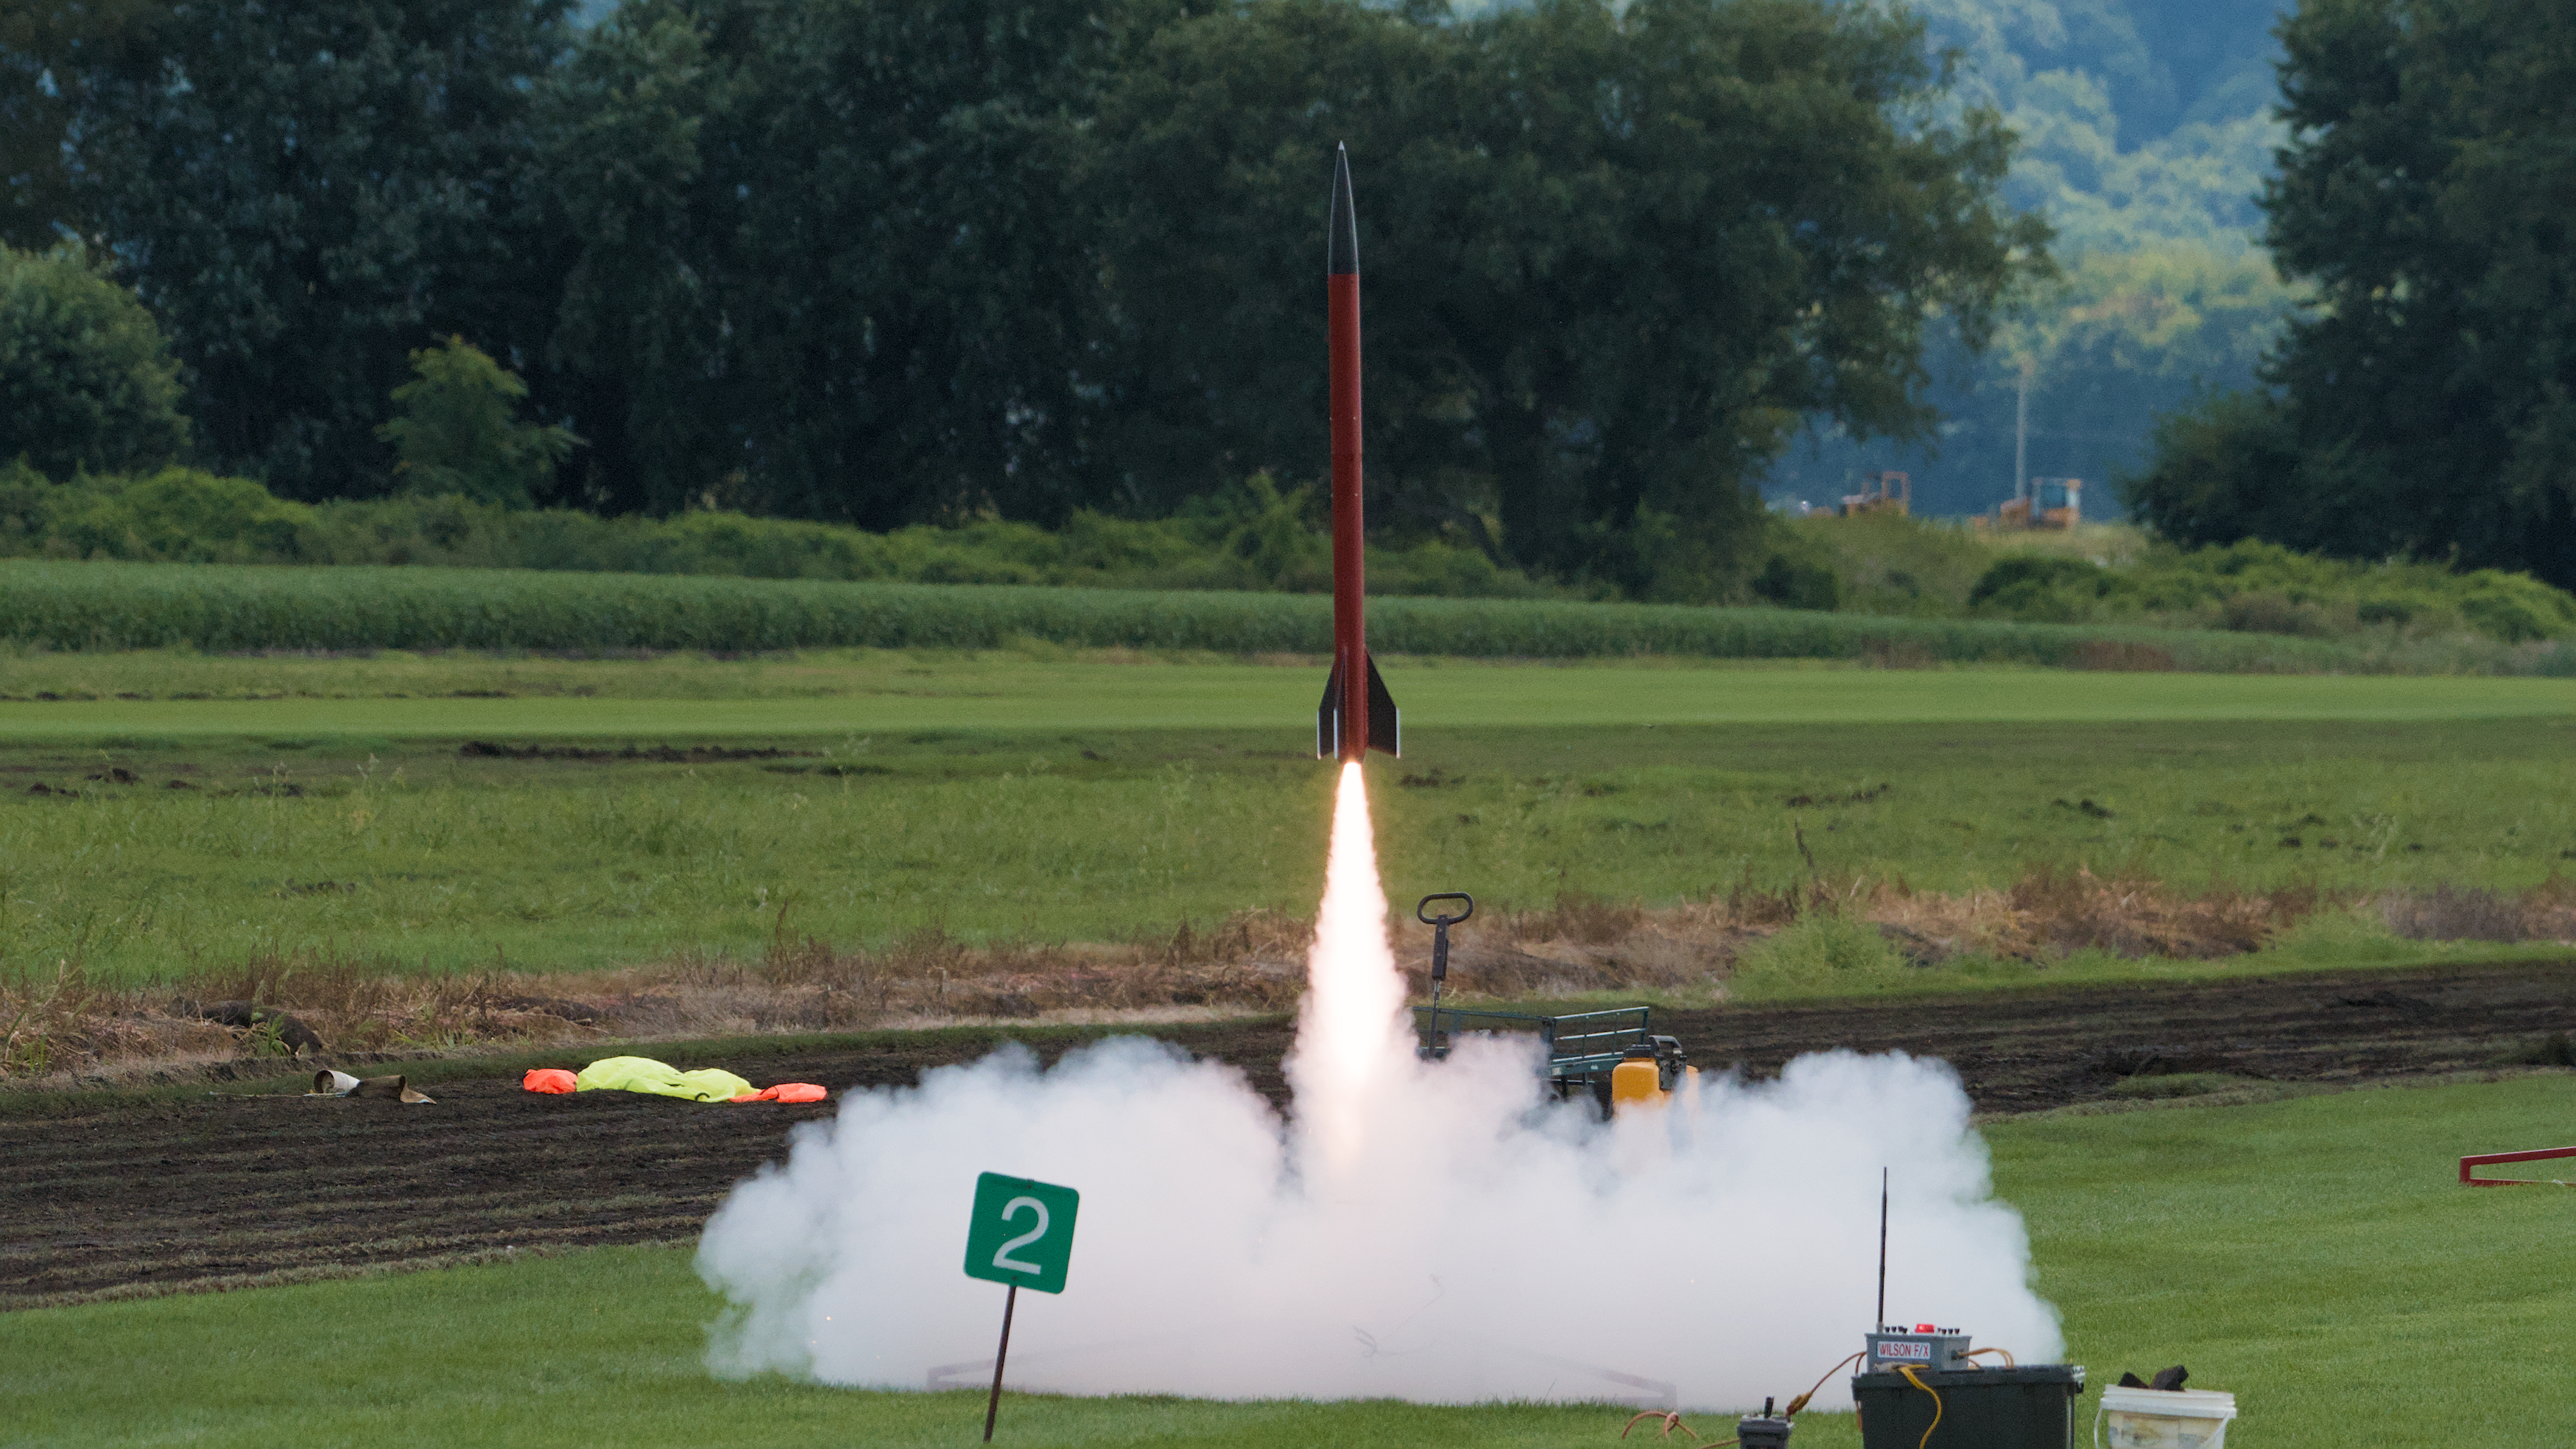
\includegraphics[trim={2cm 0 0 0}, clip,width=1\linewidth]{Documentation//ARES/Cover_Photo.jpg}
    \label{fig:placeholder}
\end{figure}
        

    \vfill
    \author[Kyle Eckert,
    \author[Nicholas Krupa,
    \author[Liam Gordon
    \vfill

    Technical Advisors\\Dr. Patricia Mellodge, Professor Allan Penda, Professor Loel Goldblatt \vfill
    Instructors\\Dr. Ying Yu, Dr. Xin Shen, Professor Jean Goulart\vfill
    \today

    \newpage
    
\end{center}
}{%
\begin{titlepage}
\centering
\vspace*{1.15in}
{\LARGE\bfseries AURORA Rocket and Experimental Systems\\[5pt] (A.R.E.S.)\par}
\vspace{0.48in}
{\Large System Functional Block Diagrams and\\ Key Principles / Technology Investigations\par}
\vspace{0.85in}
{\large\bfseries Team Members\par}\vspace{0.14in}
Nicholas Krupa --- Electrical Engineering\\[8pt]
Kyle Eckert --- Electrical Engineering\\[8pt]
Liam Gordon --- Mechanical Engineering\\[18pt]
University of Hartford --- AURORA Rocketry Club\\[18pt]
November 2026
\vfill
\end{titlepage}
}

\section{Use Case}
\subsection{Overview}
The AURORA Rocket and Experimental Systems (\ares{}) project is a modular, student-developed high-power sounding rocket for the 2027 International Rocket Engineering Competition (IREC). The vehicle is designed to approach 10,000~ft above ground level (AGL) while carrying experimental hardware in a 6-in-diameter airframe. Three electrical systems support the mission: \deimos{} collects flight measurements and provides telemetry, \phobos{} evaluates an electronically steered phased-array antenna, and \comet{} controls dual-parachute recovery.

The project also provides a research platform for the University of Hartford's AURORA Rocketry Club in collaboration with the Multiscale Metamaterial Research Laboratory. The \phobos{} payload extends the laboratory's work in microwave and antenna technologies from bench testing to a moving flight vehicle. The goal is to collect useful RF and flight data, safely recover the equipment, and establish hardware that can be improved for future student research.

\subsection{Practical Scenario}
The primary users are AURORA student engineers and University of Hartford faculty researchers. The planned 2027 IREC launch in Midland, Texas, provides a realistic setting for testing the rocket's telemetry, experimental RF payload, and recovery electronics. Ensign-Bickford Aerospace \& Defense (EBAD) supports development of the rocket, while the NASA Connecticut Space Grant Consortium supports development of the \phobos{} payload.

Before launch, the team verifies power, sensors, radio links, recovery continuity, and the installation of the subsystems. During ascent, \deimos{} measures position and orientation and transmits telemetry to a ground station. At the same time, \phobos{} varies the phases of its antenna elements to study directional communication as the rocket moves and rotates. \comet{} monitors flight events and commands the recovery sequence, with the drogue intended to deploy at apogee and the main parachute at a proposed 700~ft AGL. Following recovery, the team compares logged flight and RF measurements with predicted results. The mission is successful only if the vehicle is recovered safely and the experiment produces useful data, not merely if the altitude target is reached.

\section{Updated Requirements}
The following are preliminary design targets, not verified performance results. Final flight and RF configurations must meet the applicable IREC rules and relevant safety and communications regulations \cite{irecRules,fcc15247,faaRockets}.

\subsection{Vehicle and Integration}
\begin{itemize}
\item Target 10,000~ft AGL in the IREC 10k COTS category using an approximately 12-ft-long, 6-in-diameter fiberglass vehicle.
\item Provide removable mounting, power access, and reliable connections for the three electrical systems.
\item Support an independent commercial deployment altimeter alongside the student-developed \comet{} controller.
\item Safely recover the rocket and experimental payload for inspection and reuse.
\end{itemize}

\subsection{\deimos{} --- Tracking and Telemetry}
\begin{itemize}
\item Fit within the nose cone on a removable sled with a target assembly mass below 200~g.
\item Record GPS position, barometric altitude, acceleration, and attitude; target a 20-Hz data log.
\item Provide a battery-powered, onboard-stored telemetry record, including during radio dropouts.
\item Use a proposed 915-MHz LoRa radio and demonstrate a minimum 4-km link target, subject to the competition band plan and FCC review.
\end{itemize}

\subsection{\phobos{} --- Phased-Array Payload}
\begin{itemize}
\item Fit within the 6-in airframe, a 22-in length allocation, and a 2-kg payload mass target.
\item Operate from a proposed 9-V battery supply using separate control and antenna/RF boards.
\item Use a 2.4-GHz patch array with independently adjustable element phases for directional transmission.
\item Evaluate steering across a proposed $\pm45^\circ$ range. The initial $\sim$2-km communication target must be reevaluated against the full 10,000-ft flight geometry.
\item Verify transmitted power, antenna gain, and emission characteristics against the applicable FCC and IREC requirements rather than assuming a universal 1-W limit.
\end{itemize}

\subsection{\comet{} --- Dual-Parachute Deployment}
\begin{itemize}
\item Detect flight events using pressure and inertial sensing, independently of a ground radio link.
\item Provide separate drogue and main deployment outputs, continuity indication, external arming, and onboard logging.
\item Command the drogue near apogee and the main at a proposed altitude of approximately 700~ft AGL.
\item Verify the deployment sequence and electrical outputs through supervised ground testing before flight.
\end{itemize}

\section{System Functional Block Diagrams}
% Add these individual files to Documentation/Pics/ in Overleaf.
% The three figure environments and labels are intentionally retained.

\subsection{\phobos{} Phased-Array Antenna System}
\begin{figure}[H]
\centering
\showfbd{Documentation/Pics/PAA_Block_Diagram.png}{Phased-array control, RF distribution, phase shifters and antennas}
\caption{\phobos{} phased-array antenna functional block diagram.}
\label{fig:PAA_Block}
\end{figure}

\subsection{\deimos{} Nose-Cone Tracking System}
\begin{figure}[H]
\centering
\showfbd{Documentation/Pics/NC_Block_Diagram.png}{Sensor inputs, processor, storage, GPS and telemetry link}
\caption{\deimos{} nose-cone telemetry functional block diagram.}
\label{fig:NC_Block}
\end{figure}

\subsection{\comet{} Dual-Parachute Deployment System}
\begin{figure}[H]
\centering
\showfbd{Documentation/Pics/DPS_Block_Diagram.png}{Flight-event sensing, arming, continuity and deployment channels}
\caption{\comet{} dual-parachute deployment functional block diagram.}
\label{fig:DPS_Block}
\end{figure}

\section{Team Technology Decisions}
After comparing the technologies below, the team favors RP2040 microcontrollers for the custom electronics because of existing board and firmware experience. The \deimos{} design retains barometric and inertial sensing with a 915-MHz LoRa link, while \phobos{} uses a 2.4-GHz array with digitally commanded phase shifts and separate RF and control boards. These choices prioritize practical development, packaging, and testability; range, steering performance, and regulatory compliance still require verification. The recovery controller will use independent power and event detection rather than depend on telemetry or payload operation.
%%%%%%%%%%%%%%%%%%%%%%%%%%%%%%%%%%%%%%%%%%%%%%%%%%%
\section{Individual Key Principles and Technology Investigations}

\subsection{Nicholas Krupa --- Electrical Engineering}
\subsubsection{Microcontroller Selection}
The microcontroller acquires sensor measurements, manages data storage, and controls peripheral devices. Selecting an MCU affects software development, timing, power requirements, and the number of sensors that can be connected. The RP2040, STM32L432, and ESP32-S3 were compared using manufacturer documentation \cite{rp2040,stm32,esp32}. The RP2040 is preferred largely because the team has already developed hardware and firmware around it.

\begin{table}[H]
\centering\small
\begin{tabular}{@{}p{0.115\linewidth}p{0.145\linewidth}p{0.21\linewidth}p{0.21\linewidth}p{0.21\linewidth}@{}}
\toprule
\textbf{Category} & \textbf{Feature} & \textbf{RP2040 (Selected)} & \textbf{STM32L432} & \textbf{ESP32-S3} \\
\midrule
\multirow{4}{*}{MCU}
 & Processing & Pro: Dual-core 133-MHz MCU. Con: No hardware FPU. & Pro: Cortex-M4, 80 MHz, with FPU. Con: Lower nominal clock rate. & Pro: Dual-core processing up to 240 MHz. Con: Greater software and power overhead. \\ \cmidrule{2-5}
 & Interfaces & Pro: SPI, I\textsuperscript{2}C, USB and PIO. & Pro: Extensive low-power peripherals. & Pro: Extensive GPIO and communication options. \\ \cmidrule{2-5}
 & Power / RF & Con: External telemetry radio required. & Pro: Suited to low-power operation. Con: External radio required. & Pro: Integrated Wi-Fi/Bluetooth. Con: Not needed for these flight links. \\ \cmidrule{2-5}
 & Team experience & Pro: Existing boards, code, and documentation. & Con: Would require firmware and PCB changes. & Con: Would require firmware and PCB changes. \\
\bottomrule
\end{tabular}
\vspace{3mm}
\caption{Microcontroller technology comparison (Nicholas Krupa).}
\label{tab:MCU_Comparison}
\end{table}

\subsubsection{Barometric Sensor Selection}
Barometric pressure provides an estimate of altitude and is an important input to flight-data analysis. A sensor must operate at the intended sampling rate and connect reliably to the MCU. The MPL3115A2 is familiar to the team, while Bosch BMP390 and BMP581 devices offer newer alternatives \cite{mpl,bmp390,bmp581}. Inertial sensing will additionally use the BNO085 and an LSM6DS-family sensor; a separate high-g accelerometer may be needed if the expected acceleration exceeds their limits \cite{bno085,lsm,adxl}.

\begin{table}[H]
\centering\small
\begin{tabular}{@{}p{0.115\linewidth}p{0.145\linewidth}p{0.21\linewidth}p{0.21\linewidth}p{0.21\linewidth}@{}}
\toprule
\textbf{Category} & \textbf{Feature} & \textbf{MPL3115A2 (Selected)} & \textbf{BMP390} & \textbf{BMP581} \\
\midrule
\multirow{3}{*}{Pressure}
 & Integration & Pro: Known code and interface from prior designs. & Pro: Digital pressure sensor. Con: New code integration. & Pro: Digital pressure sensor. Con: New code integration. \\ \cmidrule{2-5}
 & Measurement & Pro: Pressure and altitude output. & Pro: High relative precision and faster sampling options. & Pro: Low-noise measurement and high sampling-rate options. \\ \cmidrule{2-5}
 & Development & Pro: Reuses established design work. Con: Older part. & Con: Requires characterization in flight conditions. & Con: Requires characterization in flight conditions. \\
\bottomrule
\end{tabular}
\vspace{3mm}
\caption{Pressure-sensor technology comparison (Nicholas Krupa).}
\label{tab:Pressure_Comparison}
\end{table}

\subsubsection{Telemetry Radio Selection}
The telemetry radio must send useful measurements from a rapidly moving vehicle to the ground station. Range, software compatibility, data rate, and power consumption are therefore important. The existing RFM95W module is preferred over newer sub-GHz and 2.4-GHz alternatives for the first implementation, pending a complete link-budget and frequency-plan review \cite{rfm95,sx1262,sx1280}.

\begin{table}[H]
\centering\small
\begin{tabular}{@{}p{0.115\linewidth}p{0.145\linewidth}p{0.21\linewidth}p{0.21\linewidth}p{0.21\linewidth}@{}}
\toprule
\textbf{Category} & \textbf{Feature} & \textbf{RFM95W (Selected)} & \textbf{SX1262} & \textbf{SX1280} \\
\midrule
\multirow{3}{*}{Telemetry}
 & Frequency & Pro: Existing 915-MHz LoRa approach. & Pro: Sub-GHz LoRa options. & Pro: 2.4-GHz operation. Con: Shares the payload's band. \\ \cmidrule{2-5}
 & Integration & Pro: Existing team firmware and interface. & Con: Radio driver / PCB redesign. & Con: Radio driver / PCB redesign. \\ \cmidrule{2-5}
 & Performance & Pro: Long-range modulation capability. Con: Link range not yet demonstrated. & Pro: Newer power/performance options. & Pro: Higher data-rate options. Con: Different path-loss tradeoff. \\
\bottomrule
\end{tabular}
\vspace{3mm}
\caption{Telemetry radio technology comparison (Nicholas Krupa).}
\label{tab:Radio_Comparison}
\end{table}

\noindent\textbf{Selected approach:} RP2040 control, MPL3115A2 pressure measurement, complementary inertial sensors, and an RFM95W telemetry link. All sensors and radio functions still require validation under the proposed flight conditions.

\subsection{Kyle Eckert --- Electrical Engineering}
\subsubsection{Phased-Array Operating Frequency}
In a phased array, changing the phase of the signal at each antenna element steers the direction of constructive interference. Frequency affects the size and spacing of the patches, free-space path loss, and the available RF components. The team compared 915 MHz, 2.4 GHz, and 5 GHz as candidates. The 2.4-GHz band was chosen as the best packaging and implementation compromise for a six-inch rocket \cite{phased,fcc15247}.

\begin{table}[H]
\centering\small
\begin{tabular}{@{}p{0.115\linewidth}p{0.145\linewidth}p{0.21\linewidth}p{0.21\linewidth}p{0.21\linewidth}@{}}
\toprule
\textbf{Category} & \textbf{Feature} & \textbf{915 MHz} & \textbf{2.4 GHz (Selected)} & \textbf{5 GHz} \\
\midrule
\multirow{4}{*}{RF band}
 & Antenna size & Con: Large elements and spacing. & Pro: Patch sizes fit the available vehicle space. & Pro: Smaller elements and spacing. \\ \cmidrule{2-5}
 & Free-space loss & Pro: Lowest loss of the three at equal distance and gains. & Moderate loss compared with alternatives. & Con: Highest loss of the three at equal gains. \\ \cmidrule{2-5}
 & RF hardware & Pro: Common telemetry parts. Con: Large array geometry. & Pro: Broad availability of RF components. & Con: Increased fabrication and integration demands. \\ \cmidrule{2-5}
 & Overall fit & Con: Difficult array packaging. & Pro: Suitable balance of aperture and complexity. & Con: Less favorable development tradeoff. \\
\bottomrule
\end{tabular}
\vspace{3mm}
\caption{Phased-array frequency comparison (Kyle Eckert).}
\label{tab:Frequency_Comparison}
\end{table}

\subsubsection{RF Architecture and Phase Control}
A phased array requires a method of dividing the transmitted signal and controlling the phase at each patch. Digital phase shifters are preferred for repeatable MCU-controlled settings. Packaged power dividers and coaxial feeds reduce the amount of custom microwave layout required for an initial flight prototype, although their losses and phase errors still need measurement \cite{phased,wilkinson,rfLaminate}.

\begin{table}[H]
\centering\small
\begin{tabular}{@{}p{0.125\linewidth}p{0.18\linewidth}p{0.22\linewidth}p{0.22\linewidth}p{0.14\linewidth}@{}}
\toprule
\textbf{Category} & \textbf{Technology} & \textbf{Pros} & \textbf{Cons} & \textbf{Decision} \\
\midrule
\multirow{2}{*}{Phase control}
 & Analog shifter & Continuous adjustment. & Bias and calibration complexity. & Alternate \\ \cmidrule{2-5}
 & \textbf{Digital shifter} & Repeatable, MCU-commanded phase settings. & Finite phase resolution. & \textbf{Selected} \\
\midrule
\multirow{2}{*}{RF divider}
 & Printed Wilkinson & Direct PCB integration. & RF layout and EM verification required. & Alternate \\ \cmidrule{2-5}
 & \textbf{Packaged splitter} & Characterized component for a first prototype. & Insertion loss and component availability. & \textbf{Selected} \\
\midrule
\multirow{2}{*}{Patch feed}
 & Microstrip feed & Compact, planar construction. & Tight matching and layout tolerances. & Alternate \\ \cmidrule{2-5}
 & \textbf{Coaxial feed} & Flexible routing and familiar connectors. & Cable/connector loss and mechanical strain. & \textbf{Selected} \\
\bottomrule
\end{tabular}
\vspace{3mm}
\caption{Phased-array RF architecture comparison (Kyle Eckert).}
\label{tab:RF_Comparison}
\end{table}

\noindent\textbf{Selected approach:} A 2.4-GHz array with separate control and RF boards, digitally controlled phase shifters, packaged dividers, and coax-fed patches. Vector-network-analyzer, beam-pattern, link-range, and regulatory testing will be needed before claiming flight-ready performance.
%%%%%%%%%%%%%%%%%%%%%%%%%%%%%%%%%%%%%%%%%%%%
\section{Sources}
\begin{thebibliography}{99}\small
\bibitem{irecRules} Experimental Sounding Rocket Association, ``IREC Documents and Forms: Competition Rules and Design Guides.'' [Online]. Available: \url{https://www.esrarocket.org/documents-and-forms}
\bibitem{faaRockets} Federal Aviation Administration, ``Amateur Rockets: 14 CFR Part 101, Subpart C.'' [Online]. Available: \url{https://www.faa.gov/space/licenses/amateur-rockets}
\bibitem{fcc15247} Federal Communications Commission, ``47 CFR \S 15.247: Operation in the 902--928 MHz and 2400--2483.5 MHz bands.'' [Online]. Available: \url{https://www.ecfr.gov/current/title-47/section-15.247}
\bibitem{rp2040} Raspberry Pi, ``RP2040 Specifications.'' [Online]. Available: \url{https://www.raspberrypi.com/products/rp2040/specifications/}
\bibitem{stm32} STMicroelectronics, ``STM32L432KC Microcontroller.'' [Online]. Available: \url{https://www.st.com/en/microcontrollers-microprocessors/stm32l432kc.html}
\bibitem{esp32} Espressif Systems, ``ESP32-S3 Wi-Fi and Bluetooth LE SoC.'' [Online]. Available: \url{https://www.espressif.com/en/products/socs/esp32-s3}
\bibitem{mpl} NXP Semiconductors, ``MPL3115A2: Pressure Sensor with Altimetry.'' [Online]. Available: \url{https://www.nxp.com/docs/en/data-sheet/MPL3115A2.pdf}
\bibitem{bmp390} Bosch Sensortec, ``BMP390 Barometric Pressure Sensor.'' [Online]. Available: \url{https://www.bosch-sensortec.com/en/products/environmental-sensors/pressure-sensors/bmp390/}
\bibitem{bmp581} Bosch Sensortec, ``BMP581 Barometric Pressure Sensor.'' [Online]. Available: \url{https://www.bosch-sensortec.com/en/products/environmental-sensors/pressure-sensors/bmp581/}
\bibitem{bno085} CEVA, ``BNO08X Family Data Sheet.'' [Online]. Available: \url{https://www.ceva-ip.com/wp-content/uploads/BNO080_085-Datasheet.pdf}
\bibitem{lsm} STMicroelectronics, ``LSM6DSO Six-Axis Inertial Module.'' [Online]. Available: \url{https://www.st.com/en/mems-and-sensors/lsm6dso.html}
\bibitem{adxl} Analog Devices, ``ADXL375: $\pm200g$ Digital MEMS Accelerometer.'' [Online]. Available: \url{https://www.analog.com/en/products/adxl375.html}
\bibitem{rfm95} HopeRF, ``RFM95W LoRa Module.'' [Online]. Available: \url{https://www.hoperf.com/modules/lora/RFM95W.html}
\bibitem{sx1262} Semtech, ``SX1262 LoRa Transceiver.'' [Online]. Available: \url{https://www.semtech.com/products/wireless-rf/lora-connect/sx1262}
\bibitem{sx1280} Semtech, ``SX1280 2.4-GHz LoRa Transceiver.'' [Online]. Available: \url{https://www.semtech.com/products/wireless-rf/lora-connect/sx1280}
\bibitem{phased} C. Pope and I. Thomas, ``Practical Beam Steering Using a Modular X-Band Phased Array,'' Analog Devices, 2026. [Online]. Available: \url{https://www.analog.com/en/resources/technical-articles/practical-beam-steering-using-modular-x-band-phased-array.html}
\bibitem{wilkinson} Cadence Design Systems, ``Design of a Reduced Footprint Microwave Wilkinson Power Divider with EM Verification.'' [Online]. Available: \url{https://www.cadence.com/en_US/home/resources/application-notes/microwave-wilkinson-power-divider-em-verif-awr-an.html}
\bibitem{rfLaminate} Rogers Corporation, ``Selection of PCB Materials for 5G.'' [Online]. Available: \url{https://rogerscorp.com/-/media/project/rogerscorp/documents/articles/english/advanced-connectivity-solutions/selection-of-pcb-materials-for-5g.pdf}
\end{thebibliography}
\end{document}